\chapter{Packet Processing Systems}
\label{chapter:packet-processing-systems}
\todo[inline]{TODO: refactor this chapter and write the introduction}
% and then describe the measurement setup required to obtain reference values for the simulation model. Two different measurements will be done, one to measure the communication latencies, and another to measure the memory latencies and throughput.

\section{Fast path Architecture}
Fully packet based architectures are becoming more common in every part of the data communication networks. This, together with the introduction of increasing Ethernet speeds introduces strict requirements to the electronic network elements. While the control- and management planes will require non-trivial solutions, the main bottleneck, to keep up with the scalability of optical transmission technology, seems to be the data plane processing.~\cite{Hauger:2009:PP}

The comparison of the speeds of Ethernet based transport networks and the processor speeds gives a perspective of the data path processing requirements. A typical Ethernet link with 100Gbps speed and minimum frame size of 64 bytes, leaves the packet processing system 6.7ns to process each packet. Completely software based solutions are insufficient to answer these requirements.~\cite{Hauger:2009:PP}

Fast path architecture refers to a path through a computer program, which incorporates smaller number of instructions or other optimization methods, compared to the 'normal path'. In packet processing systems, only minority of the data require complex processing. Thus, the data plane processing is often split into two layers: fast path and slow path.~\cite{cavium:2010:fundamentals, 6wind:2016:FP}

The typical slow path of the data plane is run on top of an operating system stack. The fast path layer processes packet outside the operating system environment, often with hardware acceleration, thus avoiding the overheads occuring from the thick software stack. This leaves only a small number of packets, that require special processing, to be forwarded to the slow path able to do more complex processing. Typical examples of packets requiring slow path handling are IP options and ARP packets. In MPSoC packet processing systems, such as Cavium OCTEON II CN6880, the processing cores can often be dynamically configured to run fast path or slow path.~\cite{cavium:2010:fundamentals, 6wind:2016:FP}

Commodity software and multi-core hardware can reduce the cost and provide high flexibity in the development and management of software packet processing, while at the same time achieving the performance of traditional hardware routers. This is achieved by replacing the thick software networking stack of commodity operating systems with special driver and kernel improvements.

Different frameworks, such as Data Plane Development Kit~\cite{Intel:DPDK}, Open vSwitch~\cite{Pfaff:2009:OVS}, and Open Event Machine~\cite{OpenEM}, have been implemented to ease the development of high speed packet processing application for commodity hardware.

\subsection{Data Plane Development Kit}
The Data Plane Development Kit (DPDK) provides a clean application programming interface and a set of coherent libraries and drivers, for Intel x86 processors. It has a generic support for many CPU's and network interface controllers ranging from Intel Atom processors to Intel Xeon processors. It supports system with and without non-uniform memory access (NUMA), and any number of processing cores.~\cite{Intel:DPDK:Doc}

DPDK runs as a Linux user-space application, utilizing the pthread library. Similarly to many other packet processing frameworks, DPDK implements a run-to-completion model, to minimize the process switching overhead. The model removes the typical operating system scheduler, and all the devices must be accessed by polling, thus eliminating the interrupt overhead. The packets can be passed between the cores, enabling more efficient and flexible core usage.~\cite{Intel:DPDK:Doc}

DPDK's Environment Abstraction Layer (EAL) abstracts the hardware environment from applications and libraries, enabling hardware agnostic implementation of packet processing applications. EAL provides services such as core affinity and assignment procedures, memory management, atomic and lock operations, and bus accesses, and interrupt handling. These features are exposed as a programming libraries.~\cite{Intel:DPDK:Doc}

DPDK has an active ecosystem around it, with wide vendor support. It is also well documented and includes several software examples demonstrating the best practices for data plane architectures, application profiling, and performance tuning.~\cite{Intel:DPDK:Doc}

\subsection{Open Event-Machine}
Open Event Machine (OpenEM) is an event-driven programming framework for multicore dataplane applications, developed by Nokia Solutions and Networks (NSN). It has been designed to ease the implementation of event/packet processing applications for different MPSoC devices. One of main drivers for the development of OpenEM has been easy integration with modern hardware accelerators.

The key concepts of OpenEM framework are execution objects, events, queues, and the scheduler. \emph{Execution objects} are the main building blocks the OpenEM application. They are the run-to-completion functions, describing the processing logic of the application. Each execution object has one or more \emph{queues} attached to it. The \emph{scheduler} selects the events from the queues, based on the global interralations of the queues. When the event is selected from the queue, the corresponding execution object is attached to the processing core, and the event is passed to it as a parameter. Once the execution object finishes its run, the scheduler chooses a new event from the queues similarly.

From the programmer's perspective, OpenEM's event-driven programming model relates closely to actor based programming models such as Erlang~\cite{Armstrong:1993:Concurrent} and Akka framework~\cite{Akka}. While the use cases for these frameworks are different, and thus cannot directly be compared with OpenEM, it is worth mentioning their message passing support. Support for combined inter-node and intra-node parallelism has potential benefits for efficient scaling in the future. HCMPI~\cite{Chatterjee:2013:HCMPI} is an example of experimental framework that combines task-parallelism with message passing. OpenEM's current specification does not support inter-node message passing.

\section{Cavium OCTEON II CN6880}
\label{sec:cavium-octeon}
%https://www.reddit.com/r/networking/comments/2kamp1/eli5_why_are_cavium_chipsets_so_popular_with

Cavium Octeon II CN6880 is a 32 MIPS core network processing unit, optimized for high-performance, high-bandwidth, and low power consumption software-defined control-plane~\cite{control-plane} and data-plane~\cite{data-plane} applications.

CN6880 provides several hardware acceleration units for enhanced packet processing and minimized software development complexity. The packet management accelerators offload the actual packet processing cores from many general packet receive, buffering, buffer management, flow classification, quality of service, and transmit processing. The accelerator functions can be customized using software, and accessing the configuration registers.~\cite{cavium:2010:fundamentals}

The packet input processor unit (PKI) and input packet data unit (IPD) work together to manage the received packets, and to perform required processing before scheduling the packets to application cores. Together they can handle most of the processing requirements of all the way through layer 2 to layer 7 in the standard OSI model~\cite{ISO:1994:OSI}. Once the required computation is done, the PKI unit sends the packet's work entry to the SSO unit to be scheduled for processing.~\cite{cavium:2010:fundamentals}

The packet transmission is handled by the packet transmission unit (PKO). When a core finishes a packet processing, it notifies the PKO that the packet is ready for transmission. The PKO then directly copies the packet data from the shared memory into its internal memory, optionally computes checksums for the packet header, transmits the packet, and optionally frees the packet data from the memory.~\cite{cavium:2010:fundamentals}

One of the key features of the CN6880 is its scheduling/synchronization and order unit (SSO). It frees the actual packet processing applications, running on the 32 MIPS cores, from the complex packet scheduling and ordering tasks. The cores execute a loop, and when a core is ready for the next packet, it requests work from the SSO, which then schedules the next work based on the quality of service priority and work group.~\cite{cavium:2010:fundamentals}

The SSO also provides efficient locking mechanisms for protecting the critical regions without explicit software locking, and allows packet processing to be done in parallel or atomically, while still maintaining the packet flow order. The processing cores can also be dedicated for specific flows. One of our goals is to be able to model the scheduling functionality with PSE, as it is crucial to the packet latency and throughput when processing several flows at the time.~\cite{cavium:2010:fundamentals}

The memory latencies have large effect in the packet processing times. The CN6880 provides several memory policies for optimized multi-core packet processing. Each of the 32 cores have dedicated 32KB L1 data and 37KB L1 instruction cache, and a shared 4MB L2 cache. The L1 data cache provides a hybrid write-through, write-back policy, using a write buffer mechanism, and the L2 cache implements a write-back policy. Several other cache related features are offered, for example to avoid unnecessary data writes after the packet transmission, and to automatically send the received packet header to L2 cache and the packet data to main memory, bypassing the L2 cache.~\cite{cavium:2010:fundamentals}

\section{Characteristic Measurements}
\label{sec:characteristic-measurements}

For the model to represent the packet latencies and throughput with enough accuracy, the model needs to be filled with apposite entity parameters. Some of the model parameters are simple enough to be obtained directly from~\cite{cavium:2010:fundamentals}, while others are either unavailable, or are presented in an unusable form to be used in the simulation model. The missing communication and memory related parameters are obtained by conducting measurements on the real CN6880 hardware. These are discussed in the following sections, respectively.

% We believe that, by determining the latecies of input phase and output phase, the behaviour of memory, and modeling the packet scheduler with enough accuracy, the sought applications' effects to the packet latencies and throughput come up with enough accuracy.

% For our approach to be valid, i.e. the abstraction of the communication latencies to be precise enough, we have to assume the fastpath is not the bottleneck in the processing phase. This assumption is reasonable because ...

% \fixme{
%   TODO:
%   \begin{itemize}
%   \item because the fastpath hardware is optimized for this task
%   \item find reference
%   \item maybe justify the stuff with some kind of rough back-of-the-envelope calculation?
%   \end{itemize}
% }

\subsection{Communication Latencies}
\label{sec:communication-latencies}

By communication latencies, we refer to the time in the input and output phase of the packet processing, between physical receive/transmit ports and the actual core processing, as described in the Section~\ref{sec:cavium-octeon}. We will include the times spent in the SSO unit for both of these metrics, as due to our resource constraints, we were unable to do the measurements with the required detail to break down these delays. Also, for our modeling purposes, it is accurate enough to assume that the input and output phases consume equal amount of processing time.

The input and output phase latencies are measured by generating traffic from external machine, and passing it through two CN6880 units back to the generator itself. The measurements were done at two independent points in the processing path, to validate the accuracy of the measurements.

\begin{figure}[]
  \begin{center}
    \includegraphics[width=\textwidth]{images/comm-measurement-setup.pdf}
    \caption{The setup used to measure the communication latencies. The communication between the nodes, packet processing on the main cores, and the input and output processing, are marked with the dashed arrows, solid black arrows, and orange arrows respectively. The probes present the points of measurement.}
    \label{fig:comm-setup}
  \end{center}
\end{figure}

In figure~\ref{fig:comm-setup}, the rectangles represent three different computing units (traffic generator, forward unit, and swap unit), and the probes present the points of time measurements. The traffic generator is a typical desktop computer running Ubuntu operating system, and the traffic was generated by Mausezahn~\cite{mausezahn}. Both of the Octeon CN6880 units are running Linux operating systems.

The packet is first generated at the packet generator and sent to the forward unit at time $t^{d}_{0}$. Forwarding unit receives the packet at time $t^{r}_{10}$, does the required processing and forwards the packet to the swap unit at time $t^{d}_{10}$. The swap unit receives the packet at time $t^{r}_{2}$, does the same processing as the forward unit (except with different destination address), and forwards the packet back to the forward unit at time $t^{d}_{2}$. Finally the forward unit receives the packet at time $t^{r}_{11}$ and forwards it to the traffic generator at time $t^{d}_{11}$, which marks it received at time $t^{r}_{0}$. The time $t_{f}$ spent in the input and output phase of one unit is then

\begin{equation}
  \label{eq:1}
  t_{f} \approx \frac{t^{r}_{11} - t^{d}_{10} - (t^{d}_{2} - t^{r}_{2})}{2}.
\end{equation}

We measured the times for packet sizes of 64B, 128B, 256B, 512B, 1024B, and 1500B, repeating the measurement for each packet 10000 times. Figures~\ref{fig:comm-latency-boxplot} and~\ref{fig:comm-latency-histograms} present the statistics of the resulting times $t_{f}$ for the different packet sizes.

\begin{figure}[]
  \begin{center}
    \includegraphics[width=\textwidth]{images/comm-latency-boxplot.pdf}
    \caption{Latency of the input and output phase of the CN6880 unit. On each box, the central mark is the median, the edges of the box are the 25th and 75th percentiles. 99.3\% of the points lie within the whiskers, and the most extreme points are presented as red crosses. Both of the axes are on logarithmic scale.}
    \label{fig:comm-latency-boxplot}
  \end{center}
\end{figure}

\begin{figure}[]
  \begin{center}
    \includegraphics[width=\textwidth]{images/comm-latency-histograms.pdf}
    \caption{Latency frequency histograms for each packet size, along with a normal density function with parameters, estimated with maximum likelihood method from the data.}
    \label{fig:comm-latency-histograms}
  \end{center}
\end{figure}

As shown in the figure~\ref{fig:comm-latency-boxplot}, the time spent in the input and output phase of the unit is roughly linear regarding to the packet size. The variation of the data is relatively small on all packet sizes. The trend of the latency with respect to the packet size, corresponds to the trend of the values measured with at the external traffic-generator (which causes $3.1\mu s$ constant overhead regardless of the packet size). The corresponding plots for the external traffic-generator measurements are omitted for clarity.

As seen from both of the figures~\ref{fig:comm-latency-boxplot} and ~\ref{fig:comm-latency-histograms}, there exist points with unexpectly large deviation from the rest of the group. These deviations seem to be independent of the packet size, and thus we assume that they are caused by the scheduling unit (SSO). This behaviour is also statistically incorporated in the simulation model.

The only packet size dependent operations in the input and output phases are the memory transfers done for the actual packet data between the memory (L2/RAM) and PKI or PKO. All the other other operations are done based on the packet header, thus requiring constant amount of time regardless of the packet size.

Since We cannot make a distinction between the input and output phase, in the simulation model presented further, we will adjust the input/output phase amount so that they consume the PKI and PKO units for the amount that corresponds the constant term of equation~\ref{eq:1}. The variable (non-constant) term is caused by the memory copies in the input/output phases, and are proportional to the packet size.

The input and output delays used in the simulation model are estimated by fitting a linear model to the data, using least square estimate. The determination coefficient of the estimate $R^2 = 0.997$. The delay for the input and output phase are divided evenly, resulting in

\begin{equation}
  \label{eq:1}
  t_{in} = t_{out} = \frac{1}{2}(0.0018\frac{\mu s}{B} * packet\_size + 1.036\mu s).
\end{equation}

\subsection{Memory Characteristics}
\label{sec:memory-characteristics}

Memory delays were measured using Multi-core Processor Architecture and Communication (MPAC) benchmarking library~\cite{Jamal:2009:MPAC}. Both, latency and throughput, were measured using different dataset sizes and number of threads. Each of the tests were run on 200,000 repetitions.

\begin{figure}[]
  \begin{center}
    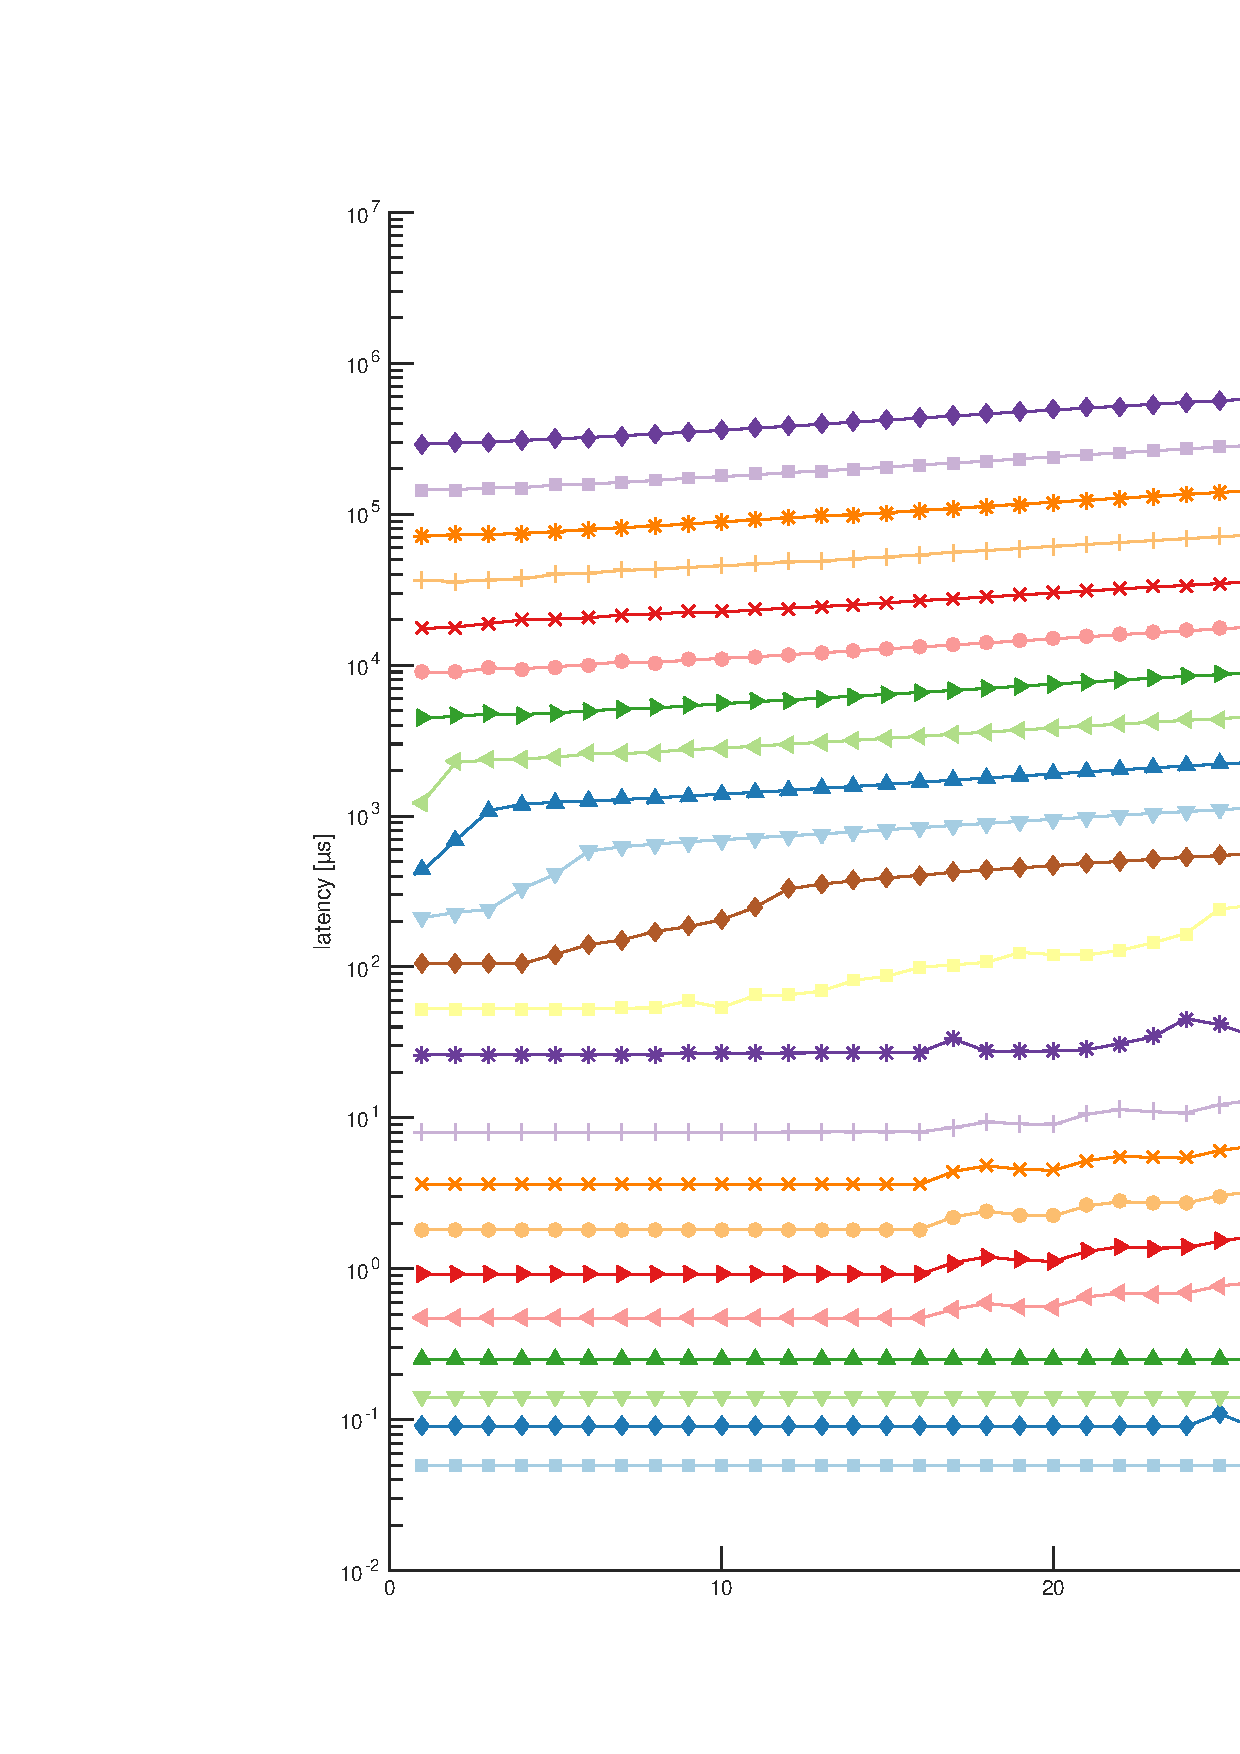
\includegraphics[width=\textwidth]{images/mem-latency.pdf}
    \caption{Memory latency of the CN6880 in microseconds across number of threads for integer data type (32bit), measured by MPAC. Each data point in the graph present one experiment run with different thread and write sizes. The latencies for different packet sizes are marked with colors as shown in the legend (in bytes). The y-axis is presented in logarithmic scale.}
    \label{fig:mem-latency}
  \end{center}
\end{figure}

Figure~\ref{fig:mem-latency} presents the results from the latency measurements for different packet sizes and thread counts. Notice that the y-axis the graph is logarithmic. As expected, the memory latencies grow together with the size of the write. The transition between the memory levels (32K L1, 4MB L2~\cite{cavium:2010:fundamentals}) can be seen as the jumps in the latency graph. With 128B - 1KB write sizes both the read and write arrays fit in the L1 cache (32KB~\cite{cavium:2010:fundamentals}), and thus the latency per repetition is independent of the thread count. With write sizes above 2KB, some of the writes hit L2 cache (4MB~\cite{cavium:2010:fundamentals}), increasing the latency as the thread count increases. Similarly, the step from L2 cache to RAM can be seen 128KB, 256KB, 512KB, 1MB, and 2MB write sizes, where both write and read arrays completely fit in the L2 cache with 8, 4, 2, 1 and 1 threads, and move to RAM beyond that.

The write latencys also thrash beyond 32 threads, especially for the cache sizes. This does not affect the main core memory accesses in the model, as only 32 threads are used for packet processing. However, these numbers work as a reference when modeling the memory communication of other units such as SSO.

\begin{figure}[]
  \begin{center}
    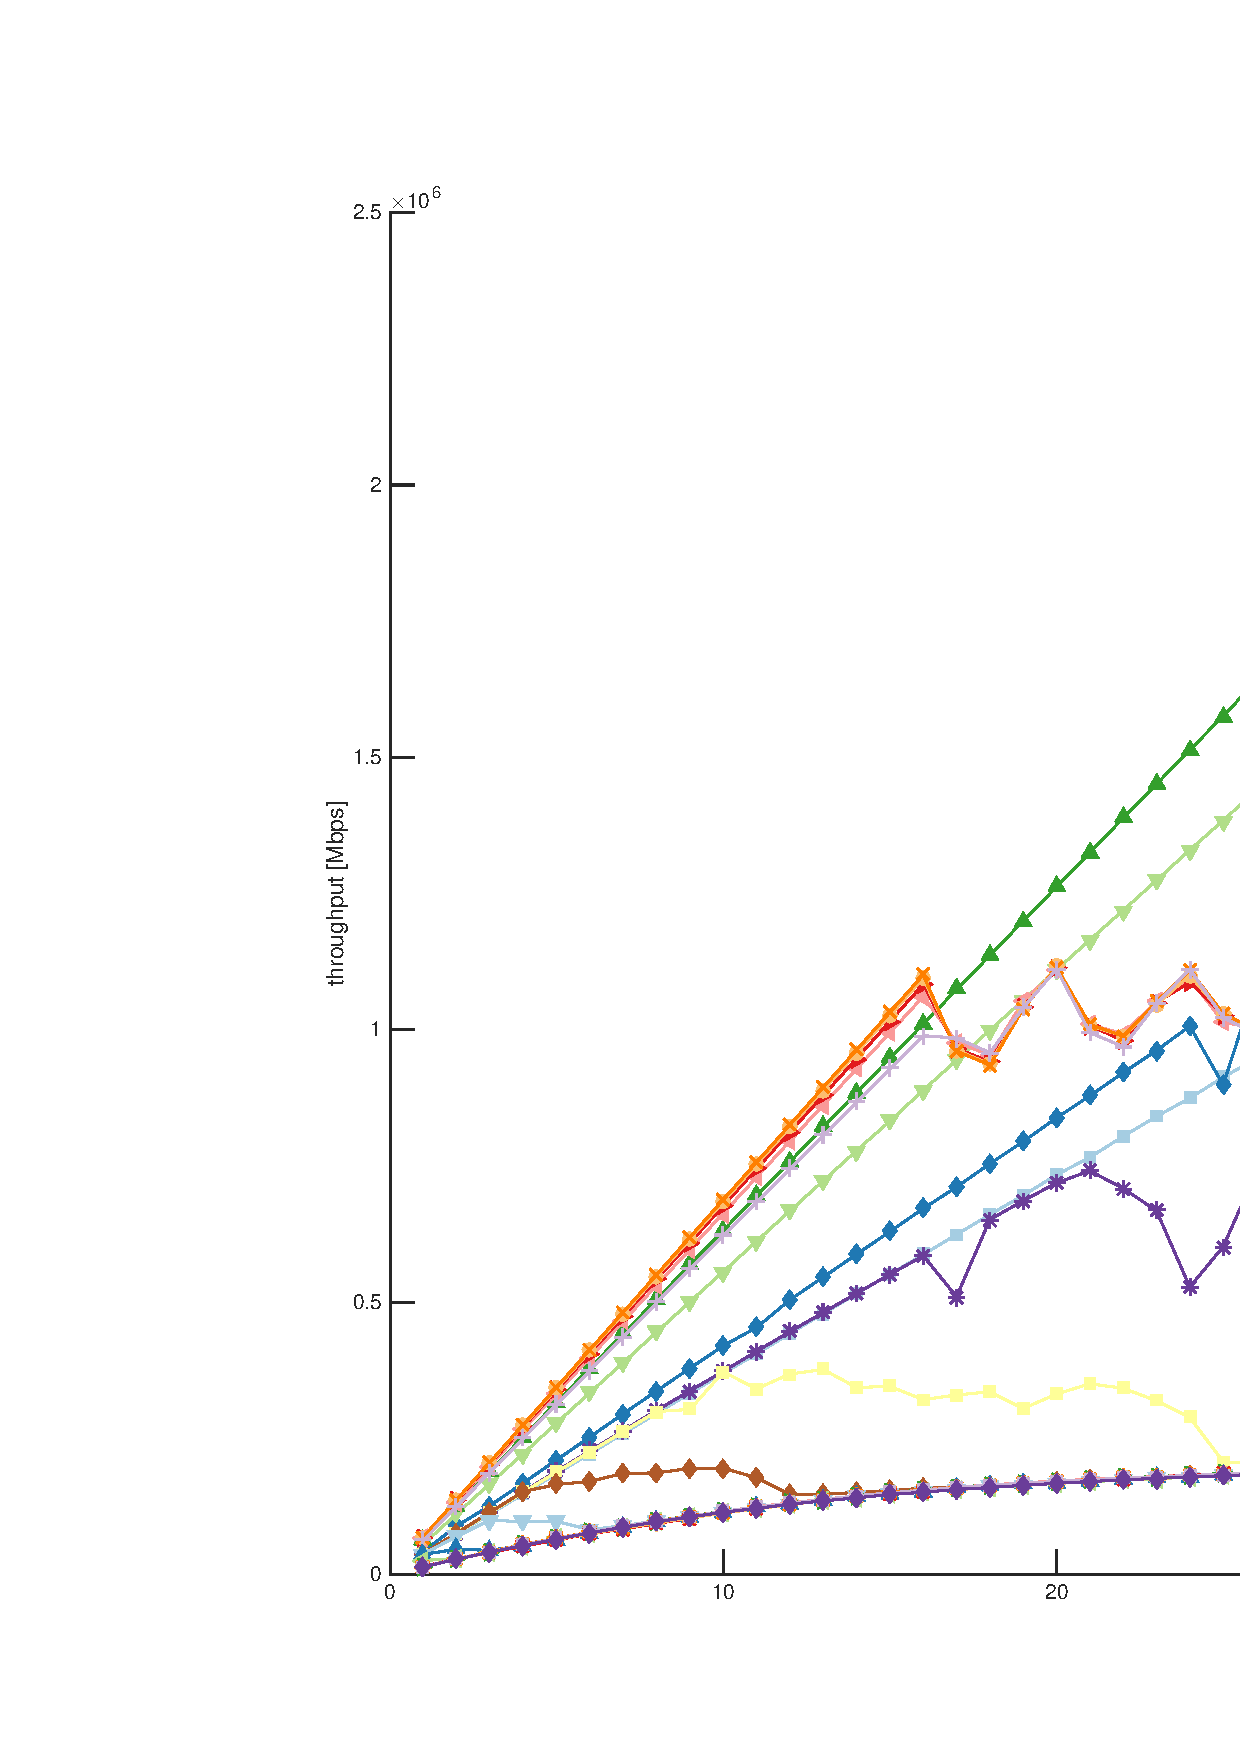
\includegraphics[width=\textwidth]{images/mem-throughput.pdf}
    \caption{Memory throughput of the CN6880 in Gbps across number of threads for integer data type (32bit), measured by MPAC. Each data point in the graph present one experiment run with different thread and data sizes. The throughput for different packet sizes are marked with colors as shown in the legend (in bytes).}
    \label{fig:mem-throughput}
  \end{center}
\end{figure}

Figure~\ref{fig:mem-latency} presents the results from the throughput measurements for different packet sizes and thread counts. Again, as expected, the maximum throughput is achieved with 1KB write lengths and 32 cores, when both the write and read arrays fit in the caches. The write throughput scales linearly with 128B - 1KB write sizes for up to 32 cores, with 2KB - 64KB up to 16 cores, and for 256KB, 512KB, and 1MB, write sizes up to 8, 4, and 2 cores respectively. The transition between the memory levels are similar as in the latency graph. Again, a clear thrashing can be seen with more than 32 threads.


%%% Local Variables:
%%% mode: latex
%%% TeX-master: "thesis-hartikainen"
%%% End:
